\documentclass[../../Thesis.tex]{subfiles}
\usepackage[italian]{babel}

\begin{document}
\chapter{Metodologia}
Questa sezione descrive in dettaglio l'approccio seguito per affrontare il problema della classificazione degli smart contracts. Questo capitolo \`e fondamentale per comprendere come sono stati raccolti, pre-processati e utilizzati i dati, quali e come sono stati configurati e addestrati i modelli e quali strumenti e tecniche sono stati impiegati per ottenere i risultati presentati.

La metodologia adottata in questa tesi \`e suddivisa nelle seguenti fasi principali:
\begin{enumerate}
    \item Raccolta e preparazione dei dati: esplorazione del dataset utilizzato, delle tecniche di pre-processing applicate e delle modalit\`a di suddivisione dei dati per l'addestramento e la valutazione.
    \item Modellazione: descrizione dell'architettura dei modelli utilizzati, delle scelte di configurazione e delle strategie di addestramento.
\end{enumerate}
Ogni fase sar\`a trattata in modo dettagliato, evidenziando le scelte metodologiche compiute e le motivazioni alla base di tali scelte. Questo approccio  garantisce trasparenza e replicabilit\`a del lavoro svolto, consentendo ad altri  di comprendere e, eventualmente, replicare i risultati ottenuti.
    
\section{Esplorazione dei dati}
\label{sec:eda}
La prima fase, quando ci si approccia ad un problema che riguarda la costruzione di modelli e l'analisi di dati \`e sicuramente l'analisi esplorativa dei dati. Questa fase \`e fondamentale per comprendere meglio la struttura del dataset e dei contratti da classificare, per individuare eventuali problemi e per ottenere una visione d'insieme dei dati. A livello pratico, questa fase di analisi esplorativa dei dati \`e stata eseguita utilizzando il linguaggio Python, con l'ausilio di librerie come Pandas, NumPy, Matplotlib e Seaborn per l'analisi e la visualizzazione dei dati.

Il dataset \cite{rossini2022slitherauditedcontracts} utilizzato in questo progetto \`e un dataset disponibile pubblicamente sulla piattaforma HuggingFace. Hugging Face \`e una piattaforma e una comunit\`a dedicata all'intelligenza artificiale, nota soprattutto per la sua vasta raccolta di modelli pre-addestrati per il linguaggio naturale, computer vision e altri compiti legati all'IA. Questa piattaforma \`e diventata una risorsa fondamentale per gli sviluppatori ed i ricercatori che lavorano nell'ambito del machine learning grazie alla sua libreria nominata ``Transformers" (che verr\`a utilizzata in questo lavoro), che offre un'implementazione semplice e potente di alcuni dei modelli pi\`u avanzati nel campo del NLP (Natural Language Processing). Hugging Face non solo fornisce modelli pre-addestrati, ma incoraggia anche la collaborazione e la condivisione all'interno della comunit\`a attraverso il suo hub online, dove gli utenti possono accedere, condividere e collaborare su modelli, dataset e altri componenti relativi all'IA. Inoltre, Hugging Face supporta un ecosistema di strumenti e risorse open-source che facilitano lo sviluppo e l'implementazione di soluzioni basate su IA.

Questo dataset contiene informazioni su ben 106.474 Smart Contracts pubblicati sulla rete Ethereum. Il dataset \`e stato costruito a partire dalla lista Smart Contracts verificati forniti da Smart Contract Sanctuary, una risorsa online che fornisce una lista verificata di Smart Contracts. Successivamente, il codice sorgente dei contratti intelligenti \`e stato scaricato sia dal suddetto repository che tramite Etherscan e poi appiattito utilizzando lo strumento di appiattimento dei contratti Slither. Il bytecode \`e stato scaricato utilizzando la libreria Web3.py, in particolare la funzione web3.eth.getCode(). Infine, ogni Smart Contract \`e stato analizzato utilizzando il framework di analisi statica Slither. Lo strumento ha individuato 38 diverse classi di vulnerabilit\`a nei contratti raccolti e sono stati quindi mappati su 6 etichette. Questi mapping sono stati derivati seguendo le linee guida del Decentralized Application Security Project (DASP) e del Smart Contract Weakness Classification Registry. Ogni entry del dataset \`e composta da quattro feature:
\begin{itemize}
    \item  \textbf{Address}: l'indirizzo del contratto
    \item  \textbf{SourceCode}: il codice sorgente del contratto, scritto in linguaggio Solidity
    \item  \textbf{ByteCode}: il codice bytecode del contratto in esadecimale, ottenuto a partire dalla compilazione del codice sorgente utilizzando il compilatore di Solidity. Questo bytecode \`e quello che viene eseguito sulla macchina virtuale di Ethereum (EVM).
    \item  \textbf{Slither}: il risultato dell'analisi statica del contratto con Slither, un tool open-source per l'analisi statica di contratti scritti in Solidity. Questo risultato \`e un array di valori che vanno da 1 a 5, dove ogni numero  rappresenta la presenza di una vulnerabilit\`a e 4 rappresenta un contratto safe, cio\`e privo di vulnerabilit\`a.
\end{itemize}
Le vulnerabilit\`a che sono state prese in questo lavoro sono le seguenti:
\begin{itemize}
    \item Access-Control
    \item Arithmetic
    \item Other
    \item Reentrancy
    \item Unchecked-Calls
\end{itemize}
 
Il dataset \`e diviso in tre sottoinsiemi: training, validation e test set.
Il dataset di training \`e composto da 79.641 contratti, il dataset di validazione da 10.861 contratti e il dataset di test da 15.972 contratti. La tabella \ref{tab:split} riassume in termini percentuali la suddivisione dei dati nei tre set.
\begin{table}[h!]
    \centering
    \begin{tabular}{|l|l|l|}
    \hline
    \textbf{Split} & \textbf{Numero di elementi} & \textbf{Percentuale} \\ \hline
    Training       & 79,641                        & 74.80\%               \\ \hline
    Validazione    & 10,861                        & 10.20\%               \\ \hline
    Test           & 15,972                        & 15.00\%               \\ \hline
    \end{tabular}
    \caption{Percentuali di ogni split rispetto al totale}
    \label{tab:split}
\end{table}
    
Tutte le informazioni sono presenti per tutti i contratti tranne l'informazione relativa al bytecode, che risulta essere assente per pochissimi contratti come visibile nella Tabella \ref{tab:no_bytecode_count}. 
\begin{table}[h!]
    \centering
    \begin{tabular}{|l|c|c|}
        \hline
        \textbf{Dataset} & \textbf{Count} & \textbf{\%} \\
        \hline
        Train & 227 & 0.285\% \\
        Test & 51 & 0.319\% \\
        Validation & 30 & 0.276\% \\
        \hline
    \end{tabular}
    \caption{Conteggio e Percentuale di Contratti Senza Bytecode per Dataset}
    \label{tab:no_bytecode_count}
\end{table}
Non ci sono valori nulli nelle altre colonne del dataset.
\subsection{Analisi delle Lunghezze dei contratti}
Per ottenere una visione d'insieme delle lunghezze dei contratti, abbiamo calcolato la lunghezza media del source code e del bytecode. Prima del preprocessing le lunghezze medie di SourceCode e ByteCode sono rispettivamente di 3155 token e 8114 token.

L'inclusione delle lunghezze medie fornisce un punto di riferimento utile per interpretare le distribuzioni e confrontare i singoli esempi di codice rispetto alla media del dataset. Queste analisi sono fondamentali per le successive fasi di preprocessing e modellazione, garantendo che i modelli possano gestire efficacemente la variabilit\`a presente nei dati.\\
Sul bytecode non \`e stato applicato nessun tipo di preprocessing per ridurre la dimensione dei dati, poich\`e essendo il codice esadecimale prodotto direttamente dal compilatore Solc di Solidity, esso \`e gi\`a nella forma pi\`u compatta possibile e non richiede ulteriori operazioni di riduzione delle dimensioni.\\
D'altro canto, per quanto riguarda il codice sorgente sono stati eliminati tutti i commenti e le funzioni getter monoistruzione, cio\`e tutte quelle funzioni \texttt{getX()} le quali abbiano come unica istruzione una istruzione di return, poich\`e sono state assunte come funzioni corrette. L'eliminazione di queste stringhe \`e avvenuta tramite una ricerca delle stringhe effettuata con una regex.\\
Abbiamo unito i set di dati di addestramento, test e validazione in un unico DataFrame per analizzare le lunghezze del source code e del bytecode. In particolare, sono state calcolate rispettivamente le lunghezze del codice sorgente e del bytecode. Effettuando le rimozioni dei commenti la media del numero di token del sourcecode scende a 1511 token, mostrando come la rimozione dei commenti abbia un grande impatto sulla lunghezza media del codice. Rimuovendo anche le funzioni getter monoistruzione la lunghezza media del source code scende a 1481 token. Abbiamo visualizzato la distribuzione delle lunghezze del source code utilizzando un istogramma. Per migliorare la leggibilit\`a del grafico, abbiamo raggruppato i dati per quanto riguarda il source code in intervalli di 500 token. L'istogramma \`e accompagnato da una linea che indica la lunghezza media dei token rappresentata con una linea tratteggiata rossa, mostrata rispettivamente nelle Figure \ref{fig:sourcecode_length_distribution} e \ref{fig:bytecode_length_distribution}.\\
\begin{figure}[htbp]
    \centering
    \begin{subfigure}[b]{0.49\textwidth}
        \centering
        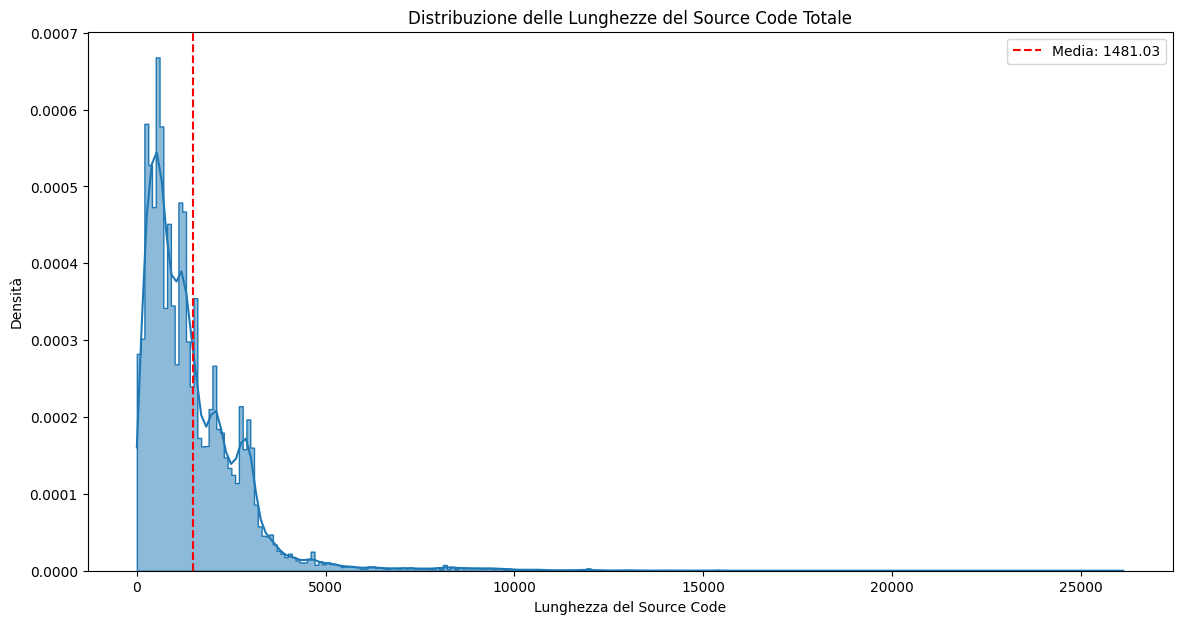
\includegraphics[width=\textwidth]{../../img/SCTokensPreprocessed.png}
        \caption{Distribuzione delle Lunghezze del Source Code dopo il preprocessing}
        \label{fig:sourcecode_length_distribution}
    \end{subfigure}
    \hfill
    \begin{subfigure}[b]{0.49\textwidth}
        \centering
        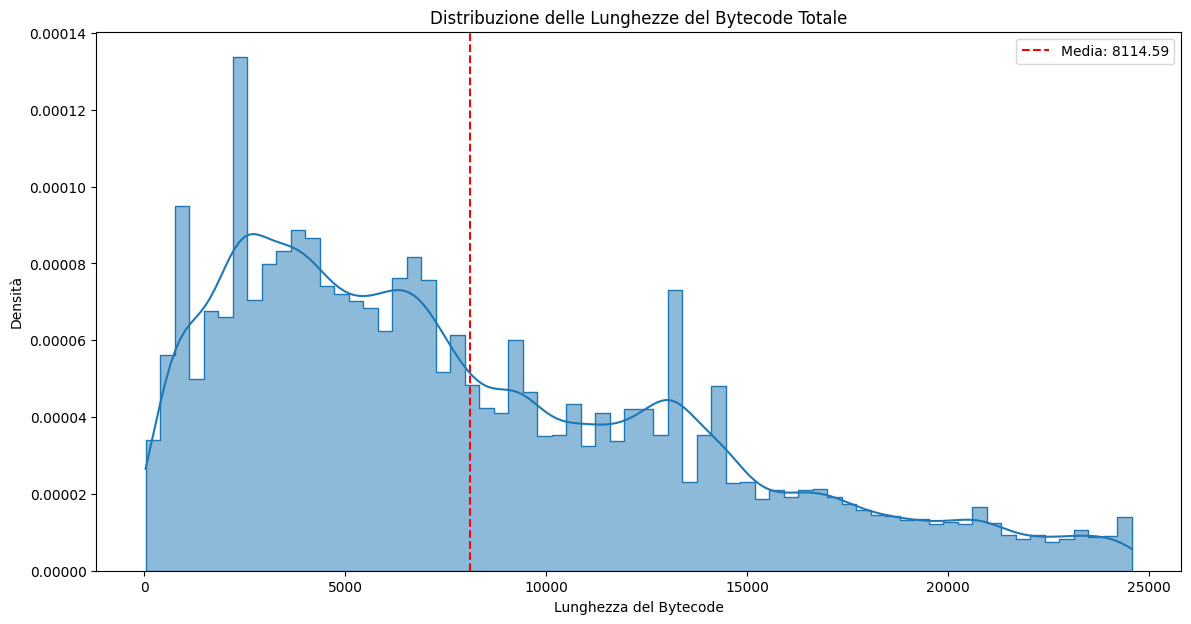
\includegraphics[width=\textwidth]{../../img/BCTokensPreprocessed.png}
        \caption{Distribuzione delle Lunghezze del Bytecode dopo il preprocessing}
        \label{fig:bytecode_length_distribution}
    \end{subfigure}
    \caption{Distribuzioni delle lunghezze del source code e del bytecode.}
    \label{fig:length_distributions}
\end{figure}
La media \`e un indicatore molto utile per guadagnare informazioni sulla lunghezza dei nostri contratti, ma potrebbe essere facilmente influenzato da valori estremi. Per questo motivo, \`e importante considerare anche la mediana, che rappresenta il valore centrale di un insieme di dati ordinati. La mediana del source code \`e di 1147 token, mentre la mediana del bytecode \`e di 6733 token. Entrambi i valori dimostrano come i contratti siano in generale, formati da sequenze molto lunghe.
Poich\`e successivamente andremo a classificare i contratti con dei modelli nella famiglia BERT che prendono in input sequenze di token lunghe al massimo 512 token abbiamo calcolato la percentuale di contratti che non superano questa soglia e in alcuni suoi multipli, per capire quanti contratti riusciamo a classificare per intero e quanti verranno invece troncati. I risultati sono mostrati nella Tabella \ref{tab:summary}.
\begin{table}[h!]
    \centering
    \begin{tabular}{|l|c|c|c|c|}
        \hline
        \textbf{Metrica} & \textbf{Sotto 512} & \textbf{Sotto 1024} & \textbf{Sotto 1536} & \textbf{Media} \\
        \hline
        \textbf{Source Code (\%)} & 21.90 & 46.04 & 64.77 & 62.21 \\
        \textbf{Bytecode (\%)} & 1.56 & 6.31 & 8.75 & 58.69 \\
        \hline
    \end{tabular}
    \caption{Percentuale di contratti sotto varie lunghezze in token.}
    \label{tab:summary}
\end{table}


Diventa per\`o importante notare, che per molti casi di contratti che superano i 5000 token questi sono cos\`i lunghi poich\`e riportano in calce al contratto anche il codice sorgente di librerie esterne, che non sono di interesse per la classificazione delle vulnerabilit\`a. 


\subsection{Distribuzione delle Classi e Matrici di Co-occorrenza}
Successivamente, la fase di esplorazione dei dati ha previsto l'analisi delle classi di vulnerabilit\`a dei dati. In questa sezione, presentiamo la distribuzione delle classi e le matrici di co-occorrenza per i dataset di addestramento, test e validazione. Si precisa che i risultati di seguito proposti si riferiscono gi\`a al dataset da cui sono stati sottratti i contratti privi di bytecode.

\subsubsection{Distribuzione delle Classi}

La Tabella \ref{tab:class_distribution} mostra la distribuzione delle classi per i tre dataset. \`e evidente che la classe ``unchecked-calls" \`e la pi\`u frequente in tutti e tre i dataset, mentre la classe ``access-control" \`e la meno rappresentata.
\begin{table}[h!]
    \centering
    \begin{tabular}{|l|c|c|c|c|c|c|c|c|}
        \hline
        \textbf{Class} & \multicolumn{2}{|c|}{\textbf{Train}} & \multicolumn{2}{|c|}{\textbf{Test}} & \multicolumn{2}{|c|}{\textbf{Validation}} & \multicolumn{2}{|c|}{\textbf{Full}} \\
        \cline{2-9}
        & \textbf{Count} & \textbf{\%} & \textbf{Count} & \textbf{\%} & \textbf{Count} & \textbf{\%} & \textbf{Count} & \textbf{\%} \\
        \hline
        access-control & 11619 & 8.71\% & 2331 & 8.71\% & 1588 & 8.73\% & 15538 & 8.72\% \\
        arithmetic & 13472 & 10.10\% & 2708 & 10.12\% & 1835 & 10.09\% & 18015 & 10.10\% \\
        other & 20893 & 15.67\% & 4193 & 15.67\% & 2854 & 15.69\% & 27940 & 15.67\% \\
        reentrancy & 24099 & 18.07\% & 4838 & 18.09\% & 3289 & 18.08\% & 32226 & 18.08\% \\
        safe & 26979 & 20.23\% & 5405 & 20.20\% & 3676 & 20.21\% & 36060 & 20.23\% \\
        unchecked-calls & 36278 & 27.21\% & 7276 & 27.20\% & 4951 & 27.21\% & 48505 & 27.21\% \\
        \hline
    \end{tabular}
    \caption{Distribuzione delle Classi nei Dataset di Addestramento, Test, Validazione e Completo}
    \label{tab:class_distribution}
\end{table}

Le Figure \ref{fig:relative_distribution} e \ref{fig:absolute_distribution} mostrano rispettivamente la distribuzione percentuale e assoluta delle classi nell'intero dataset. Queste visualizzazioni forniscono una panoramica chiara della frequenza delle diverse classi all'interno del dataset, evidenziando le differenze di distribuzione tra le classi.
\begin{figure}[h!]
    \centering
    \begin{subfigure}[b]{0.45\linewidth}
      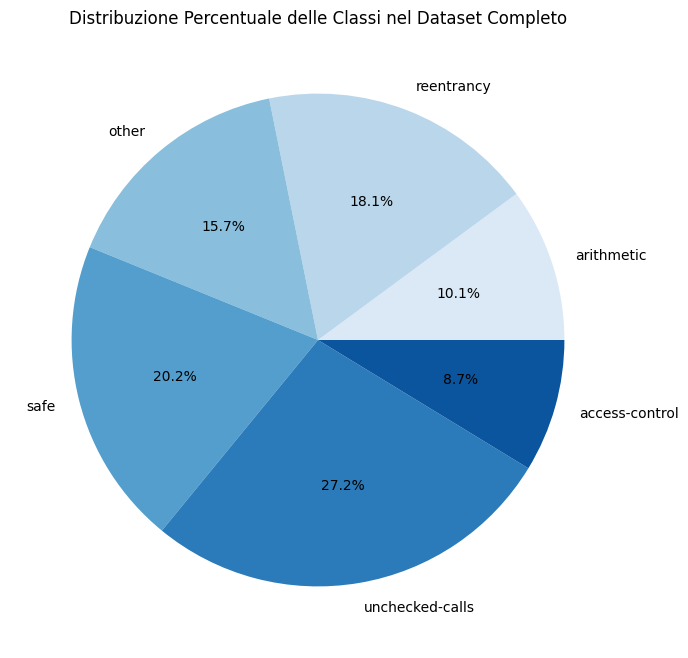
\includegraphics[width=\linewidth]{../../img/class-distribution-relative.png}
      \caption{Distribuzione Percentuale delle Classi}
      \label{fig:relative_distribution}
    \end{subfigure}
    \hspace{0.5cm}
    \begin{subfigure}[b]{0.45\linewidth}
      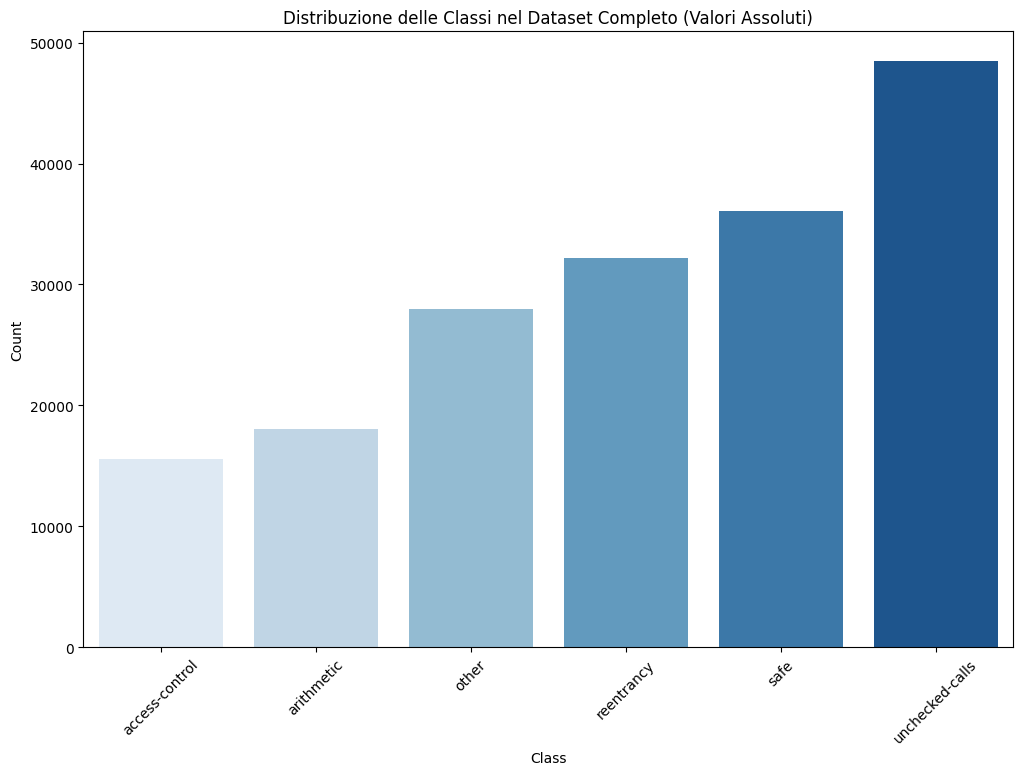
\includegraphics[width=\linewidth]{../../img/class-distribution-absolute.png}
      \caption{Distribuzione Assoluta delle Classi}
      \label{fig:absolute_distribution}
    \end{subfigure}
    \caption{Distribuzioni delle Classi nell'intero dataset, in termini relativi e assoluti.}
    \label{fig:class_distributions}
  \end{figure}
  Dalla distribuzione delle classi nei diversi dataset, possiamo osservare che:

  \begin{itemize}
      \item Le classi sono distribuite in modo abbastanza uniforme nei dataset di addestramento, test e validazione, con percentuali simili tra i tre split per classe
      \item La classe `unchecked-calls' \`e la pi\`u frequente in tutti e tre i dataset.
      \item La classe `access-control' \`e la meno frequente.
      \item Le classi `safe' e `reentrancy' sono anche abbastanza rappresentate
  \end{itemize}
\subsubsection{Matrici di Co-occorrenza}
Le Tabelle \ref{fig:train_cooccurrence_matrix}, \ref{fig:test_cooccurrence_matrix} e \ref{fig:val_cooccurrence_matrix} mostrano le matrici di co-occorrenza per i dataset di addestramento, test e validazione rispettivamente. Le matrici di co-occorrenza indicano la frequenza con cui ogni coppia di classi appare insieme nello stesso elemento.

In questa sezione, vengono presentate le matrici di co-occorrenza per ogni split del dataset, mostrando sia in termini assoluti che relativi il numero di cooccorrenze tra le varie classi.

\begin{figure}[H]
    \centering
    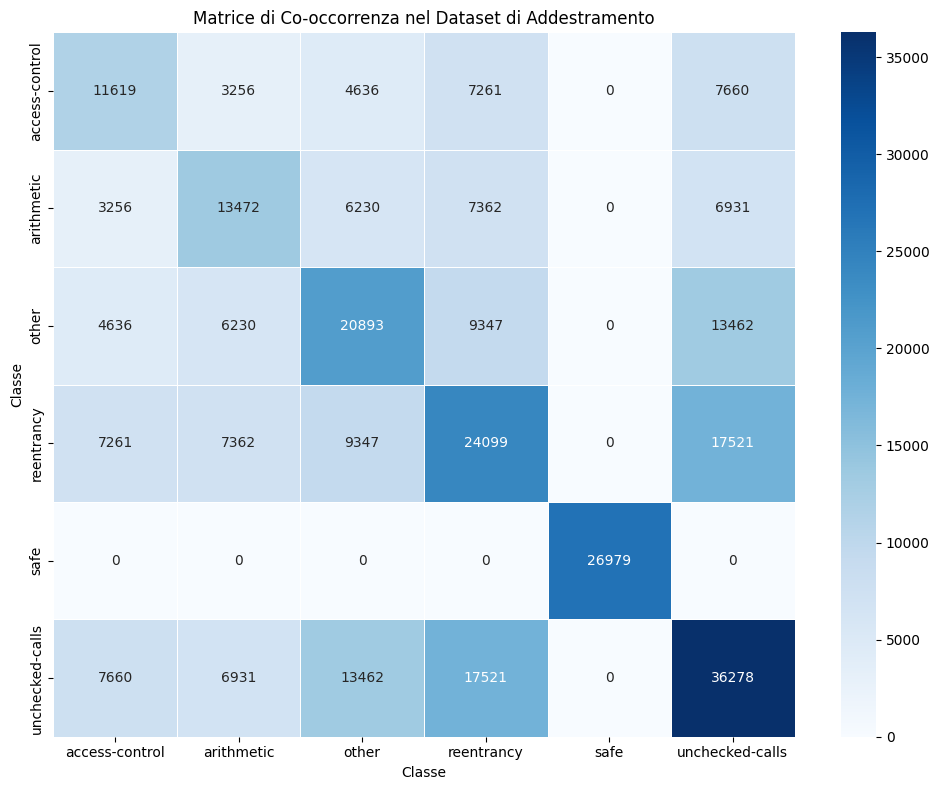
\includegraphics[width=0.7\textwidth]{../../img/TrainCo-occurrency.png}
    \caption{Matrice di Co-occorrenza nel Dataset di Addestramento}
    \label{fig:train_cooccurrence_matrix}
\end{figure}

\begin{figure}[H]
    \centering
    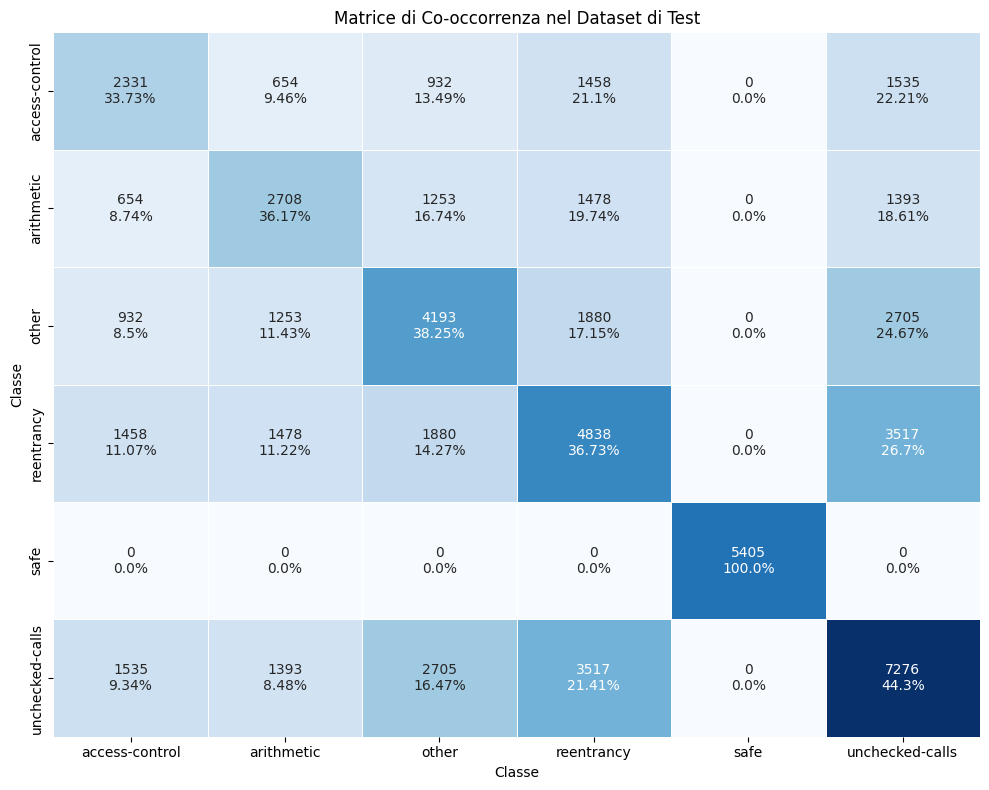
\includegraphics[width=0.7\textwidth]{../../img/TestCo-occurrency.png}
    \caption{Matrice di Co-occorrenza nel Dataset di Test}
    \label{fig:test_cooccurrence_matrix}
\end{figure}

\begin{figure}[h]
    \centering
    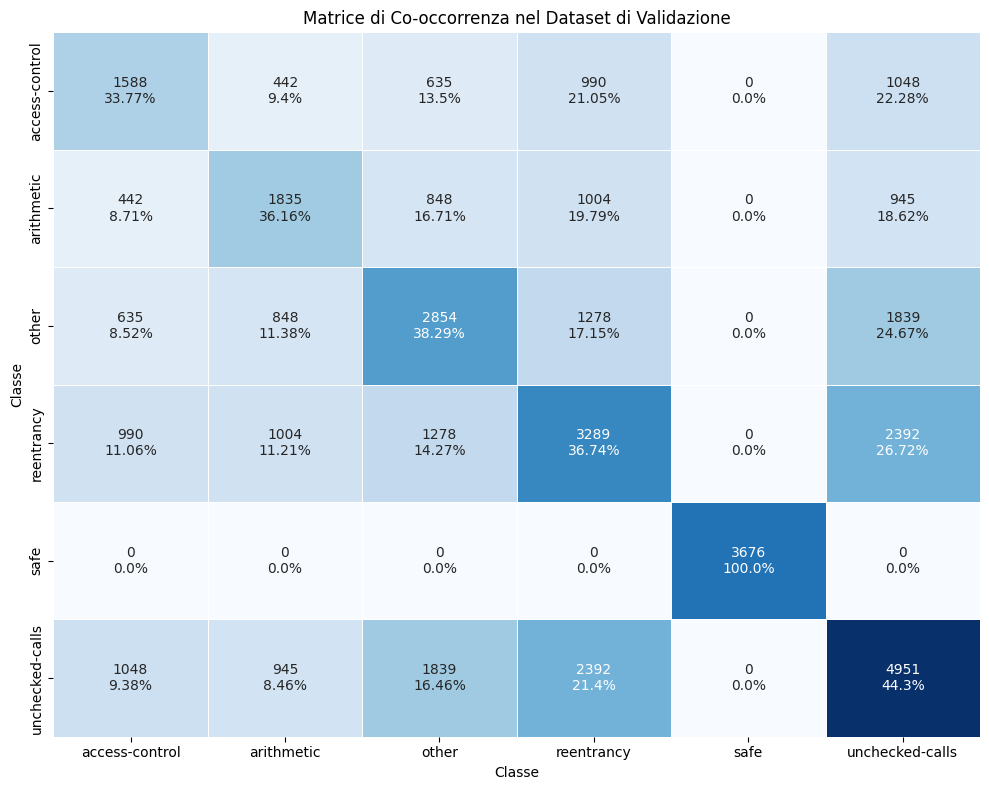
\includegraphics[width=0.7\textwidth]{../../img/ValCo-occurrency.png}
    \caption{Matrice di Co-occorrenza nel Dataset di Validazione}
    \label{fig:val_cooccurrence_matrix}
\end{figure}

Analizzando le matrici di co-occorrenza, notiamo che:

\begin{itemize}
    \item La classe safe, che rappresenta i contratti privi di vulnerabilit\`a, correttamente non appare contemporaneamente a nessuna delle altre classi. 
    \item Le classi `unchecked-calls' co-occorrono frequentemente con `reentrancy', `other', e `access-control'. Questo suggerisce che i contratti con chiamate non verificate spesso presentano anche altri tipi di vulnerabilit\`a.
    \item Le classi `arithmetic' e `reentrancy' mostrano una co-occorrenza significativa, suggerendo che le vulnerabilit\`a aritmetiche possono spesso essere associate a problemi di rientro.
\end{itemize}

Si \`e analizzata a questo punto, la percentuale di volte, per ogni classe, per cui la classe stessa appariva non come unica vulnerabilit\`a presente, ma il contratto avesse almeno un'altra vulnerabilit\`a. I risultati sono mostrati nella Tabella \ref{tab:multi_vuln}.

\begin{table}[h!]
    \centering
    \begin{tabular}{|l|c|c|}
        \hline
        \textbf{Vulnerabilit\`a} & \textbf{\%} \\
        \hline
        unchecked-calls  & 72.32\% \\
        reentrancy  & 91.51\% \\
        other  & 84.17\% \\
        arithmetic  & 77.05\% \\
        access-control  & 87.27\% \\

        \hline
    \end{tabular}
    \caption{Percentuale delle classi in cui la classe stessa non \`e l'unica vulnerabilit\`a presente.}
    \label{tab:multi_vuln}
\end{table}
Interessante \`e il risultato relativo alla classe Reentrancy, che pur non essendo la classe pi\`u presente all'interno del dataset, \`e quella che pi\`u frequentemente appare in concomitanza con altre classi di vulnerabilit\`a, allo stesso modo della classe Access-Control, che pur essendo la classe minoritaria, appare in concomitanza con altre classi di vulnerabilit\`a in una percentuale molto alta.
Questi risultati evidenziano l'importanza di considerare la co-occorrenza delle classi quando si analizzano le vulnerabilit\`a negli smart contracts, poich\`e molte vulnerabilit\`a non si verificano in isolamento ma tendono a manifestarsi insieme ad altre.


\section{Modellazione}
In questa sezione, descriviamo l'architettura dei modelli utilizzati per la classificazione degli Smart Contracts. In particolare, presentiamo i dettagli relativi ai modelli BERT utilizzati, alle scelte di configurazione e alle strategie di addestramento.
Come si evince dalla sezione precedente le feature su cui i modelli dovranno basare le loro predizioni sono il codice sorgente e il bytecode dei contratti, cio\`e dati di natura testuale. La natura dei dati fa s\`i che problema possa essere affrontato efficacemente utilizzando tecniche di elaborazione del linguaggio naturale (NLP, Natural Language Processing).

\subsection{Natural Language Processing, NLP}
L'Elaborazione del Linguaggio Naturale (NLP, da \emph{Natural Language Processing}) \`e un campo  di studi interdisciplinare che combina linguistica, informatica e intelligenza artificiale. Si occupa dell'interazione tra computer e linguaggio umano (naturale), in particolare del processamento, analisi e costruzione di modelli riguardanti grandi quantit\`a di dati linguistici naturali \cite{jurafsky2009speech}. 
Le due grandi sfide dell'NLP si possono riassumere in due grandi aree di ricerca: la comprensione del linguaggio e la generazione del linguaggio.\\
 La comprensione del linguaggio comprende compiti come l'analisi sintattica, l'analisi semantica, il riconoscimento delle entit\`a nominate e la risoluzione delle coreferenze. Questi compiti sono cruciali per la conversione del linguaggio naturale in una rappresentazione formale che le macchine possano elaborare. L'analisi sintattica, ad esempio, mira a determinare la struttura grammaticale di una frase, mentre l'analisi semantica si concentra sulla comprensione del significato del testo.\\ In secondo luogo, 
la generazione del linguaggio riguarda la produzione automatica di testo, che pu\`o includere la sintesi vocale, la traduzione automatica e la generazione di risposte automatiche in chatbot. Questo aspetto dell'NLP \`e fondamentale per creare sistemi che non solo comprendano il linguaggio umano, ma che possano anche comunicare in modo naturale e coerente con gli utenti.

Negli ultimi  anni, il campo dell'NLP ha fatto enormi progressi passando dall'epoca delle schede perforate e dell'elaborazione batch (in cui l'analisi di una frase poteva richiedere fino a 7 minuti) all'era di Google e simili (in cui milioni di pagine web possono essere elaborate in meno di un secondo) \cite{6786458}, sino ad arrivare ai giorni d'oggi con l'avvento di modelli di deep learning. Per decenni, l'approccio alla ricerca nel campo dell'NLP prevedeva l'utilizzo di modelli shallow come SVM \cite{SVM} e regressione logistica \cite{logisticReg} allenati su feature sparse e fortemente multidimensionali. Negli ultimi anni, d'altro canto,  le reti neurali basati su rappresentazioni di vettori densi hanno prodotto risultati superiori su una grande vastit\`a di task diversi nel mondo dell'NLP \cite{TrendsInNLP}. 
Lo stato dell'arte attuale nell'NLP \`e in molti task rappresentato dall'introduzione di una nuova architettura, che \`e andata a sostituire i precedenti modelli  RNN e LSTM \cite{LSTM} tradizionali, ovvero i modelli basati su Transformers, introdotti per la prima volta nel paper ``Attention is All You Need" da Vaswani et al. nel 2017 \cite{AttentionIsAllYouNeed}. I Transformer hanno rivoluzionato il campo grazie al meccanismo di self-attention, che consente al modello di valutare e ponderare l'importanza di ogni parola in una frase rispetto alle altre parole della stessa frase, indipendentemente dalla loro distanza posizionale. Questo approccio permette un'elaborazione parallela dei dati, in netto contrasto con la natura sequenziale delle RNN e degli LSTM, migliorando notevolmente l'efficienza computazionale. La struttura dei Transformer \`e organizzata in blocchi ripetuti di encoder e decoder, dove l'encoder elabora l'input costruendo una rappresentazione interna, e il decoder utilizza questa rappresentazione per generare l'output. Questa architettura ha dimostrato prestazioni eccezionali in molte applicazioni di NLP, tra cui la traduzione automatica, la comprensione e la generazione del linguaggio, la sintesi del testo e il riassunto automatico. Dall'architettura dei Transformer sono derivati molti modelli di successo, tra cui i modelli BERT, la famiglia di modelli GPT e tanti altri modelli diventati oggi lo stato dell'arte nei vari task del mondo dell'NLP. 

Di seguito illustreremo i tre modelli che sono stati utilizzati in questo lavoro, ovvero BERT, CodeBERT e DistilBERT, tutti basati sull'architettura dei Transformer.
\subsection{BERT, Bidirectional Encoder Representations from Transformers}
Il modello BERT (Bidirectional Encoder Representations from Transformers) \`e stato presentato da Devlin et al. nel 2018 \cite{BERT}. BERT \`e un modello di deep learning pre-addestrato per l'elaborazione del linguaggio naturale. BERT \`e stato allenato su un corpus di testo molto ampio, comprendente 3.3 miliardi di parole, utilizzando due task di apprendimento supervisionato: il \emph{Masked Language Model} (MLM) e il \emph{Next Sentence Prediction} (NSP). Il Masked Language Model maschera randomicamente alcuni dei token in input con l'obiettivo di predire l'id nel vocabolario della parola mascherata basandosi solo sul contesto che la circonda, considerando sia il contesto a sinistra che a destra della parola mascherata, in modo da catturare il contesto bidirezionale. Il Next Sentence Prediction, invece, prevede se una frase \`e la successiva rispetto a un'altra frase. Questo task \`e stato introdotto per insegnare al modello a comprendere il contesto e la coerenza tra le frasi. Al momento della sua pubblicazione BERT rappresentava lo stato dell'arte in ben undici diversi task nel campo dell'NLP ed \`e stato il primo modello a raggiungere state-of-the-art performance in molti task sentence-level e token-level, superando anche molte architetture specifiche per task. 

\subsubsection{Architettura}
L'architettura del modello BERT \`e un encoder bidirezionale multi-strato basato sui Transformer, come descritto nell'implementazione originale di Vaswani et al. (2017) \cite{AttentionIsAllYouNeed}. I parametri principali di un'architettura di BERT sono il numero di strati $L$, la dimensione nascosta $H$ e il numero di self-attention heads $A$. All'interno dell'architettura di BERT, due concetti fondamentali sono la \textit{hidden size} e le \textit{attention heads}.

La \textbf{hidden size} ($H$) si riferisce alla dimensione dei vettori di rappresentazione nelle varie fasi di elaborazione del modello. In termini pratici, rappresenta la dimensionalit\`a dello spazio in cui le rappresentazioni intermedie dei token vengono proiettate durante l'elaborazione nel modello Transformer. Questa dimensione influisce direttamente sulla capacit\`a del modello di catturare le informazioni a partire dai dati in input; una hidden size maggiore consente al modello di rappresentare e processare informazioni pi\`u dettagliate, a costo per\`o di un incremento dei requisiti computazionali.

Le \textbf{attention heads} ($A$) sono un componente cruciale del meccanismo di self-attention nei Transformer. Ogni attention head esegue una funzione di attenzione, ovvero calcolare un insieme di pesi che determinano l'importanza relativa di ogni token nella sequenza di input rispetto agli altri token, permettendo cos\`i al modello di concentrarsi su diverse parti della sequenza di input simultaneamente. 

La tabella \ref{tab:bert_params} riassume i parametri principali dei modelli BERT\textsubscript{BASE} e BERT\textsubscript{LARGE}, mentre un'immagine rappresentativa dell'architettura dei Transformer, di BERT\textsubscript{BASE} e BERT\textsubscript{LARGE} \`e mostrata in Figura \ref{fig:bert_input}.
\begin{table}[h]
    \centering
    \begin{tabular}{|c|c|c|c|}
        \hline
        Modello & Layers $L$ & Hidden Size $H$ & Self-Attention Heads $A$ \\
        \hline
        BERT\textsubscript{BASE} & 12 & 768 & 12 \\
        \hline
        BERT\textsubscript{LARGE} & 24 & 1024 & 16 \\
        \hline
    \end{tabular}
    \caption{Parametri principali dei modelli BERT\textsubscript{BASE} e BERT\textsubscript{LARGE}}
    \label{tab:bert_params}
\end{table}
\label{sec:bert}

BERT \`e stato preaddestrato con un embedding WordPiece \cite{WordPiece} con un vocabolario di 30.000 token. Il primo token di ogni sequenza \`e sempre un token di classificazione speciale ([CLS]). L'hidden state finale corrispondente a questo token \`e utilizzato come rappresentazione aggregata della sequenza per i task di classificazione, che \`e proprio il modo in cui BERT verr\`a utilizzato in questo lavoro. BERT pu\`o gestire pi\`u sequenze di token in input, ciascuna delle quali \`e seguita da un token speciale ([SEP]), che permette di disambiguare l'appartenenza di un token ad una sequenza piuttosto che ad un'altra. 

\begin{figure}[H]
    \centering
    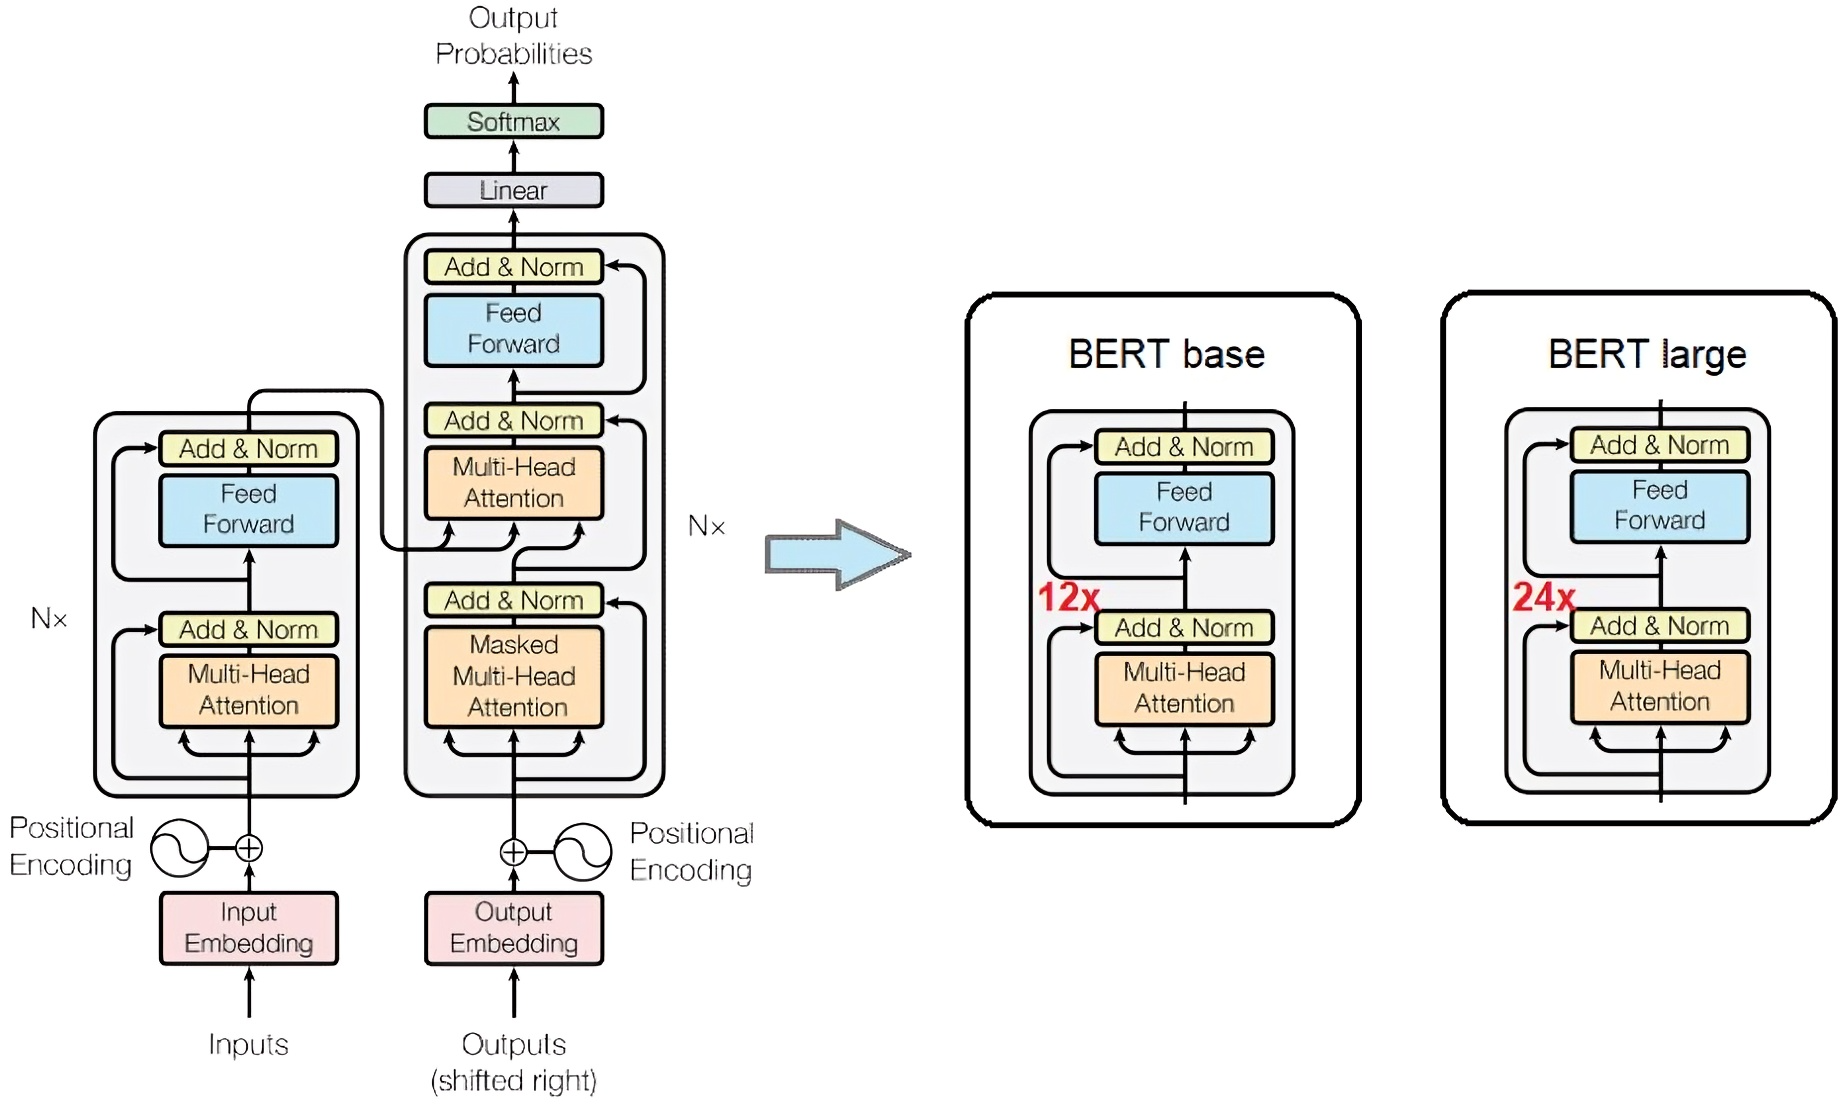
\includegraphics[width=\textwidth]{../../img/bert_base_large.png}
    \caption{Architettura di Transformers, BERT\textsubscript{BASE} e BERT\textsubscript{LARGE}. Immagine di \cite{BertImage}}
    \label{fig:bert_input}
\end{figure}

Per ogni token in input, BERT calcola un embedding che \`e dato dalla somma di tre componenti come \`e possibile vedere in Figura \ref{fig:bert_embedding}:
\begin{itemize}
    \item \textbf{Token Embeddings}: sono i vettori di embedding per ciascun token nel vocabolario. Questi embedding sono allenati durante il pre-addestramento e sono aggiornati durante il fine-tuning. BERT utilizza una tecnica chiamata Wordpiece tokenization, in cui le parole vengono
    suddivise in sottostringhe pi\`u piccole chiamate wordpieces. Questa tecnica permette di
    creare un vocabolario flessibile contenente sia parole che sotto-parole, per esempio
    prefissi, suffissi o singoli caratteri. Il vocabolario cos\`i creato \`e in grado di gestire tutte le
    possibili sequenze di caratteri e di evitare l'utilizzo di token OOV (Out Of Vocabulary) \cite{WordPiece}.
    \item \textbf{Segment Embeddings}: sono i vettori di embedding che indicano a quale sequenza appartiene ciascun token. Questi embedding sono utilizzati per distinguere tra le due sequenze di input in un task di classificazione di sequenza.
    \item \textbf{Position Embeddings}: sono una componente critica per aiutare il modello a comprendere la posizione di ciascun token all'interno di una sequenza di testo. Questi embedding consentono a BERT di distinguere tra parole con lo stesso contenuto ma posizionate in posizioni diverse all'interno della frase. Ci\`o contribuisce a catturare le relazioni tra le parole in modo pi\`u completo e consente a BERT di eccellere in una vasta gamma di compiti di elaborazione del linguaggio naturale.
\end{itemize}

\begin{figure}[H]
    \centering
    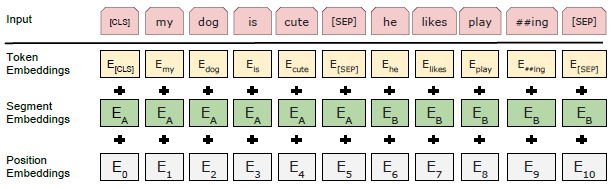
\includegraphics[width=\textwidth]{../../img/bert-input.png}
    \caption{Rappresentazione degli input di BERT. Immagine di \cite{BERT}}
    \label{fig:bert_embedding}
\end{figure}

\subsubsection{Pre-Training}
Il pre-training di BERT \`e stato effettuato usando due task di apprendimento non supervisionato: 
\begin{itemize}
    \item \textbf{Masked Language Model (MLM)}: in questo task venivano mascherate il 15\% dei token in input e si voleva far si che il modello predicesse i token mascherati. Questo processo in letteratura viene anche spesso chiamato \emph{Cloze} \cite{Taylor1953}. In questo caso i vettori dell'hidden layer finale che si riferisce al token mascherato venivano dati in input ad una funzione softmax sul vocabolario per predire il token mascherato. Per non creare troppo divario tra il pre-addestramento e il fine-tuning, durante questa fase di pre-training con MLM il token speciale [MASK] veniva utilizzato solo l'80\% delle volte, il 10\% delle volte veniva sostituito con un token casuale e il 10\% delle volte veniva lasciato il token originario.
    \item \textbf{Next Sentence Prediction (NSP)}: in molti task di NLP, come Question-Answering \`e necessario che i modelli siano in grado di comprendere relazioni tra due frasi. Per far si che il modello imparasse a riconoscere le relazioni tra frasi BERT \`e stato pre-addestrato su un task di predizione della frase successiva. Nello specifico, prese due frasi A e B il modello doveva predire se la frase B fosse la successiva rispetto alla frase A, questo nel dataset di training era vero nel 50\% dei casi. 
\end{itemize}

\subsubsection{Fine-tuning di BERT}

Il fine-tuning di BERT consiste nell'adattare il modello pre-allenato a compiti specifici, come la classificazione del testo, l'analisi del sentimento, il \textit{question answering} e altri. BERT utilizza l'architettura \textit{Transformer}, che permette di modellare relazioni complesse tra le parole di un testo grazie al meccanismo di \textit{self-attention}. Questo consente a BERT di processare sia singoli testi che coppie di testi.

Durante il fine-tuning, il modello pre-allenato viene ulteriormente addestrato su un dataset specifico del compito da risolvere, modificando tutti i parametri del modello. Questo include i pesi dei livelli di \textit{self-attention}, le rappresentazioni degli \textit{hidden layers} e i parametri degli strati di output. Ad esempio, per un compito di classificazione del testo, il token [CLS], che rappresenta l'intera sequenza, viene utilizzato per determinare la classe del testo. Per compiti a livello di token, come il \textit{named entity recognition} (NER), ogni token del testo viene etichettato individualmente.

Il processo di fine-tuning richiede meno risorse computazionali rispetto al pre-allenamento. Con l'uso di GPU o TPU, il fine-tuning pu\`o essere completato in poche ore, rendendo BERT un'opzione potente e versatile per una variet\`a di applicazioni di elaborazione del linguaggio naturale.

\subsection{DistilBERT}
Nel 2020 \`e stato presentato DistilBERT, un modello pi\`u piccolo e pi\`u veloce rispetto a BERT, sviluppato da Sanh et al. \cite{DistilBERT}. Il modello presentato dichiara che DistilBERT \`e in grado di ridurre la complessit\`a di BERT del 40\% pur mantenendo il 97\% delle prestazioni di BERT ed essere 60\% pi\`u veloce. 

I risultati di DistilBERT sono stati ottenuti grazie ad una tecnica chiamata \emph{knowledge distillation}, che \`e una tecnica di compressione in cui modello pi\`u piccolo, detto \emph{modello studente}, viene allenato per riprodurre i comportamenti di un modello pi\`u grande (o un insieme di modelli) detto \emph{modello insegnante}. Questo processo di distillazione permette di ridurre la complessit\`a del modello studente, riducendo il numero di parametri e la complessit\`a computazionale, mantenendo allo stesso tempo le prestazioni del modello pi\`u grande. Nell'apprendimento supervisionato, un modello di classificazione \`e generalmente allenato per predire l'istanza di una classi massimizzando la stima di probabilit\`a di quella label. Un modello che funziona in maniera ottima predirr\`a una probabilit\`a alta sulla classe corretta e probabilit\`a vicine allo zero per le classi errate. 

Il training del modello studente si basa su una combinazione di tecniche di distillazione del modello e di apprendimento supervisionato. Viene calcolata una  \textit{distillation loss} utilizzando le \textit{soft target probabilities} del modello insegnante. Questa perdita \`e definita come:

$$
L_{ce} = \sum_i t_i \log(s_i)
$$

dove $t_i$ (rispettivamente $s_i$) \`e una probabilit\`a stimata dall'insegnante (rispettivamente dallo studente). Questa funzione obiettivo fornisce un segnale di training ricco sfruttando l'intera distribuzione dell'insegnante. Seguendo \cite{hinton2015distilling}, viene utilizzata una \textit{softmax-temperature}, definita come:

$$
p_i = \frac{\exp(z_i / T)}{\sum_j \exp(z_j / T)}
$$

dove $T$ controlla la morbidezza della distribuzione di output e $z_i$ \`e il punteggio del modello per la classe $i$. La stessa temperatura $T$ viene applicata sia allo studente che all'insegnante durante il training, mentre in fase di inferenza, $T$ \`e impostata a 1 per tornare ad una funzione \textit{softmax} standard.

L'obiettivo finale del training \`e una combinazione lineare della distillation loss $L_{ce}$ con la loss di  training supervisionato, cio\`e la loss del \textit{masked language modeling} $L_{mlm}$. Per allineare le direzioni dei vettori hidden state del modello student e teacher \`e stata aggiunta una  \textit{cosine embedding loss}, $L_{cos}$. La Loss finale \`e quindi definita come:
$$
L = \alpha L_{ce} + \beta L_{mlm} + \gamma L_{cos}
$$

Dove $\alpha$, $\beta$, e $\gamma$ sono pesi che bilanciano i diversi termini di loss. Questa combinazione permette di mantenere la qualit\`a del modello distillato avvicinandolo il pi\`u possibile alla performance del modello insegnante.

\subsubsection{Architettura}
L'architettura del DistilBERT \`e simile a quella di BERT, ma con alcune differenze chiave. Vengono eliminati i \emph{token-type embedding} e la dimensione in termini di layer viene dimezzata. Sono state ottimizzate la maggior parte delle operazioni usate nell'architettura dei Transformer, come i \emph{linear layer} e \emph{layer normalization} ed \`e stato dimostrato che ridurre la dimensione dell'hidden state non ha un impatto significativo sulle prestazioni del modello, quindi \`e rimasta invariata. Per l'inizializzazione del modello student \`e stato utilizzato un layer del modello BERT poich\`e hanno la stessa dimensione. 

\begin{figure}
    \centering
    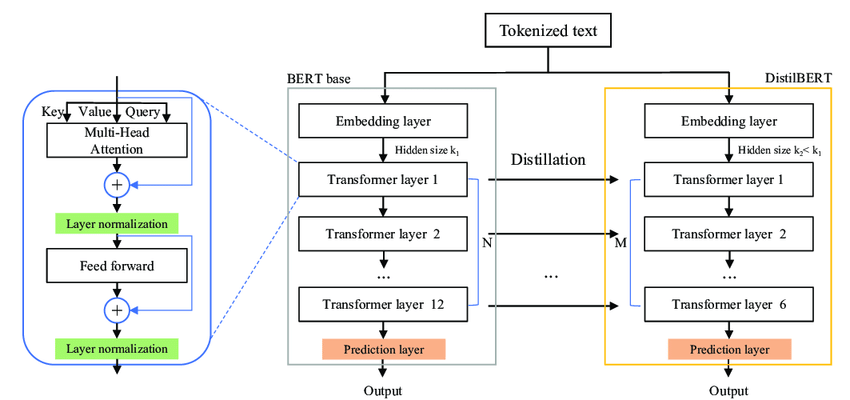
\includegraphics[width=\textwidth]{../../img/DistilBERT-Architecture.png}
    \caption{Architettura di DistilBERT. Immagine di \cite{DistilbertImage}}
    \label{fig:distilbert}
\end{figure}

\subsection{RoBERTa e CodeBERT}
A partire da BERT, nel 2019 \`e stato presentato RoBERTa (Robustly optimized BERT approach) da Liu et al. \cite{RoBERTa}. RoBERTa \`e un modello di deep learning pre-addestrato per l'elaborazione del linguaggio naturale, che migliora le prestazioni di BERT attraverso una serie di modifiche e ottimizzazioni. A livello architetturale, BERT e RoBERTa sono quasi identici, entrambi basati sull'architettura \textit{Transformer} con encoder bidirezionali. Tuttavia, le differenze principali tra i due risiedono nel processo di pre-training e nelle scelte di ottimizzazione. BERT utilizza due obiettivi di pre-training: il \textit{Masked Language Modeling} (MLM) e il \textit{Next Sentence Prediction} (NSP), mentre RoBERTa si concentra esclusivamente su MLM, eliminando l'obiettivo NSP. RoBERTa introduce anche il \textit{dynamic masking}, dove le maschere applicate ai token cambiano ad ogni epoca di training, rispetto al \textit{static masking} utilizzato da BERT. Inoltre, RoBERTa utilizza una quantit\`a di dati di training molto pi\`u grande e adotta configurazioni di iperparametri pi\`u aggressive, come dimensioni del batch maggiori e tassi di apprendimento pi\`u elevati. Queste modifiche rendono RoBERTa pi\`u efficace e robusto, migliorando le sue performance su una variet\`a di compiti di elaborazione del linguaggio naturale rispetto a BERT.


Il modello CodeBERT \`e un modello presentato per la prima volta da Microsoft nel 2020 \cite{CodeBERT}. Il modello \`e stato costruito con la stessa architettura del modello RoBERTa-base, avendo quindi un numero totale di parametri pari a 125M. 
 

\subsubsection{Fase di Pre-Training di CodeBERT}

Nella fase di pre-training, l'input \`e costituito dalla concatenazione di due segmenti con un token separatore speciale, ovvero: $$[CLS], w_1, w_2, \ldots, w_n, [SEP], c_1, c_2, \ldots, c_m, [EOS]$$
Un segmento \`e testo in linguaggio naturale e l'altro \`e codice di un determinato linguaggio di programmazione. [CLS] \`e un token speciale posizionato all'inizio dei due segmenti, la cui rappresentazione nascosta finale viene considerata come la rappresentazione aggregata della sequenza per task di classificazione o ranking. Seguendo il metodo standard di elaborazione del testo nei \textit{Transformer}, \`e stato considerato un testo in linguaggio naturale come una sequenza di parole, splittandolo utilizzando  \textit{WordPiece}. Allo stesso modo, il codice sorgente \`e stato considerato come una sequenza di token.
L'output di CodeBERT offre: 
\begin{itemize}
    \item la rappresentazione vettoriale contestuale di ciascun token, sia per il linguaggio naturale che per il codice
    \item la rappresentazione di [CLS], che funziona come rappresentazione aggregata della sequenza, allo stesso modo che in BERT.
\end{itemize}
I dati di training che sono stati utilizzati nel pretraining sono sia dati \emph{bimodali}, ovvero dati che contengono sia testo scritto in linguaggio naturale che codice di un linguaggio di programmazione, che dati \emph{unimodali}, ovvero dati che contengono solo codice senza linguaggio naturale. 

I dati sono stati raccolti da repository Github, dove un datapoint:
\begin{itemize}
    \item \emph{bimodale:} \`e rappresentato da una singola funzione a cui \`e associata della documentazione in linguaggio naturale.
    \item \emph{unimodale:} \`e rappresentato da una singola funzione senza documentazione in 
    linguaggio naturale.
\end{itemize}
Nello specifico, \`e stato utilizzato un dataset offerto da \cite{CodeBERTDataset} che contiene 2.1M di dati bimodali e 6.4M di dati unimodali suddivisi in 6 linguaggi di programmazione: Python, Java, JavaScript, Ruby, Go e PHP. Tutti i dati erano provenienti da repository pubblici e open-source su Github e sono stati filtrati sulla base cinque criteri:
\begin{enumerate}
    \item ogni progetto deve essere usato da almeno un altro progetto 
    \item ogni documentazione viene troncata al primo paragrafo
    \item le documentazioni inferiori a tre token sono state rimosse
    \item funzioni piu corte di tre linee di codice sono state rimosse
    \item le funzioni che abbiamo nel nome la sottostringa ``test" sono state rimosse
\end{enumerate}
Il pretraining di CodeBERT \`e stato effettuato utilizzando due diverse funzioni obiettivo. Il primo metodo \`e stato il MLM, che \`e stato utilizzato per preaddestrare il modello a predire i token mascherati, questo \`e stato applicato sui dati bimodali. Anche in questo caso, seguendo l'approccio usato dal modello BERT originario \cite{BERT},  sono stati mascherati il 15\% dei token tra token appartenenti al linguaggio naturale e token facenti parte del codice sorgente. Il secondo metodo applicato \`e stato il \emph{replaced token detection} che utilizza sia i dati bimodati che quelli unimodali.  Durante il pre-training, alcuni token nell'input originale, che pu\`o essere testo in linguaggio naturale o codice, vengono sostituiti con token casuali. Il compito del modello \`e quindi rilevare quali token sono stati sostituiti. Il processo funziona nel seguente modo: il modello riceve una sequenza di token contenente sia token originali che token sostituiti. Per ogni token, il modello deve prevedere una probabilit\`a che indichi se il token \`e stato sostituito o meno. L'obiettivo di training per RTD \`e minimizzare la perdita di classificazione binaria tra i token originali e quelli sostituiti. Questo metodo sfrutta l'intero contesto della sequenza, permettendo a CodeBERT di apprendere rappresentazioni pi\`u ricche e accurate sia per il linguaggio naturale che per il codice.

Per quanto riguarda il fine-tuning, allo stesso modo di BERT, CodeBERT pu\`o essere specializzato su task specifici tunando tutti i suoi parametri in modo molto efficiente. Il modello ha ottenuto performance allo stato dell'arte per task che includono ricerca di codice tramite linguaggio naturale, generazione di documentazione a partire dal codice. 


\section{Implementazione}
In questa sezione, descriveremo a livello pratico quali sono state le scelte implementative effettuate per la costruzione dei modelli di classificazione degli smart contracts, descrivendo sia il pre-processing dei dati che la costruzione e l'addestramento dei modelli, nonch\`e le librerie utilizzate. 

I tre modelli precedenti, BERT, DistilBERT e CodeBERT sono quelli scelti ed utilizzati in questo lavoro per la classificazione di vulnerabilit\`a degli smart contracts. I task di classificazione possono dividersi in tre categorie principali: 
\begin{itemize}
    \item \textbf{Classificazione Binaria:} in cui il modello deve predire se un dato elemento appartiene o meno ad una classe specifica. Facendo un esempio nel contesto degli smart contracts, un task di classificazione binaria comporterebbe la predizione della presenza o meno di vulnerabilit\`a in uno smart contract. 
    \item \textbf{Classificazione Multiclasse:} in cui il modello deve predire, all'interno di un insieme di classi, a quale classe appartiene un dato elemento, posto che possa appartenere ad una sola classe. Ad esempio, un task di classificazione multiclasse potrebbe essere quello di prevedere la vulnerabilit\`a presente in uno smart contract posto che questo possa avere un solo tipo di vulnerabilit\`a.
    \item \textbf{Classificazione Multilabel:} in cui il modello deve predire, all'interno di un insieme di classi, a quali classi appartiene un dato elemento, posto che possa appartenere a pi\`u classi contemporaneamente. 
\end{itemize}
Questo lavoro \`e stato affrontato come un task di classificazione multilabel, in quanto uno smart contract pu\`o avere pi\`u di una vulnerabilit\`a contemporaneamente. 

Il codice per il pre-processing dei dati, la costruzione, il training e la valutazione dei modelli \`e stato scritto in Python. Python \`e un linguaggio di programmazione Turing-completo ad alto livello, ampiamente riconosciuto per la sua semplicit\`a e leggibilit\`a. La vasta disponibilit\`a di librerie e strumenti specifici per l'elaborazione del linguaggio naturale e l'apprendimento automatico, come NumPy, Pandas e Scikit-learn, rende Python una scelta ideale per questo tipo di ricerca. Inoltre, Python \`e supportato da una vasta comunit\`a di sviluppatori e ricercatori, che lo rendono uno dei linguaggi pi\`u utilizzati a livello mondiale per la manipolazione di dati e per lo sviluppo di modelli di Machine e Deep Learning. In aiuto a Python \`e stata utilizzata la libreria PyTorch, una libreria di deep learning altamente performante e flessibile, sviluppata da Facebook AI Research (FAIR) \cite{Pytorch}. PyTorch offre un'interfaccia intuitiva e dinamica per la costruzione e l'addestramento di modelli di apprendimento profondo, facilitando la sperimentazione e l'ottimizzazione dei modelli. Inoltre, PyTorch \`e supportato da una comunit\`a di ricerca attiva e in crescita, che contribuisce con numerosi modelli pre-addestrati e risorse che accelerano lo sviluppo e la valutazione dei modelli. Queste caratteristiche rendono Python e PyTorch l'ovvia scelta per questo lavoro.

Fondamentali per lo sviluppo sono state altre due librerie offerte da HuggingFace, rispettivamente Transformers e Datasets. Transformers \`e una libreria open-source che offre un'implementazione di modelli di apprendimento profondo pre-addestrati, tra cui BERT, RoBERTa, DistilBERT e molti altri. Questa libreria offre un'interfaccia semplice e intuitiva per caricare, costruire e addestrare modelli di apprendimento profondo, facilitando la sperimentazione e l'ottimizzazione dei modelli. Datasets, invece, \`e una libreria open-source che offre un'interfaccia semplice e intuitiva per caricare e manipolare dataset che sono stati caricati sulla piattaforma HuggingFace. Questa libreria offre una vasta gamma di dataset pre-caricati, tra cui il dataset \cite{rossini2022slitherauditedcontracts} utilizzato in questo lavoro, semplificando il processo di raccolta dei dati. 

Di seguito, verranno presentate le tecniche utilizzate per il proceprocessing dei dati e tutti gli esperimenti effettuati e i vari modelli costruiti, i cui risultati verranno poi discussi nel capitolo \ref{chap:results} successivo.
\subsection{Pre-Processing dei Dati}
Come detto in precedenza, nella sezione dell'analisi esplorativa dei dati (vedi sezione \ref{sec:eda}), il dataset utilizzato per questo lavoro \`e stato fornito da Rossini et al. \cite{rossini2022slitherauditedcontracts}. Il dataset \`e stato ottenuto dalla piattaforma Hugginface, le quali librerie sono state utilizzate per dividere il dataset in training, validation e test set. 

Per quanto riguarda il pre-processing del codice sorgente sono state rimosse tramite espressioni regolari le parti di codice riguardanti i commenti e riguardanti le funzioni getter monoistruzione. Mostriamo ora un esempio di codice per il pre-processing del codice sorgente:
\begin{python}
    def remove_comments(string):
    pattern = r"(\".*?\"|\'.*?\')|(/\*.*?\*/|//[^\r\n]*\$)"
    # first group captures quoted strings (double or single)
    # second group captures comments (//single-line or /* multi-line */)
    regex = re.compile(pattern, re.MULTILINE|re.DOTALL)
    def _replacer(match):
        # if the 2nd group is not None, then we have captured a real comment string.
        if match.group(2) is not None:
            return ""
        else: # otherwise, we will return the 1st group
            return match.group(1)
    return regex.sub(_replacer, string)
\end{python}
Dopo aver rimosso anche le funzioni getter monoistruzione, il codice sorgente viene passato ad un tokenizer, il cui compito \`e trasformare il testo in una serie di token, ossia unit\`a fondamentali come parole, sottoparole o caratteri. Il tokenizer di BERT utilizza la tecnica WordPiece per segmentare il testo, frammentando le parole rare in sottoparole pi\`u comuni e preservando il contesto originale. Il tokenizer di CodeBERT, specializzato per il codice sorgente, riconosce le sintassi dei linguaggi di programmazione e segmenta il codice in token significativi.

Il processo di tokenizzazione include i seguenti passaggi:

\begin{itemize}
    \item \textbf{Padding}: Quando le sequenze di token hanno lunghezze diverse, si utilizza il padding per uniformare la lunghezza delle sequenze al valore massimo prestabilito. Vengono aggiunti token speciali (di solito uno zero) alle sequenze pi\`u corte fino a raggiungere la lunghezza desiderata. Questo \`e essenziale per creare batch di dati di dimensioni uniformi per l'elaborazione parallela.
    
    \item \textbf{Token IDs}: Ogni token viene convertito in un ID numerico univoco in base al vocabolario del tokenizer. Questi ID sono utilizzati dal modello per eseguire l'elaborazione e l'analisi del testo. Per esempio, la parola ``hello" potrebbe essere convertita nell'ID 123, mentre ``world" potrebbe corrispondere all'ID 456.
    
    \item \textbf{Attention Mask}: La maschera di attenzione \`e un array di valori binari che indica quali token devono essere considerati dal modello durante l'addestramento o l'inferenza. I token reali ricevono un valore di 1, mentre i token di padding ricevono un valore di 0. Questo permette al modello di ignorare i token di padding durante il calcolo dell'attenzione.
\end{itemize}

Di seguito viene riportato un esempio di implementazione di una classe \texttt{CustomDataset} in Python, che utilizza un tokenizer per preparare il codice sorgente per l'input del modello:

\begin{python}
class CustomDataset(Dataset):

    def __init__(self, dataframe, tokenizer, max_len):
        self.tokenizer = tokenizer
        self.data = dataframe
        self.sourceCode = dataframe["source_code"]
        self.targets = dataframe["label"]
        self.max_len = max_len

    def __len__(self):
        return len(self.sourceCode)

    def __getitem__(self, index):
        sourceCode = str(self.sourceCode[index])
        sourceCode = " ".join(sourceCode.split())

        inputs = self.tokenizer.encode_plus(
            sourceCode,
            None,
            add_special_tokens=True,
            max_length=self.max_len,
            pad_to_max_length=True,
            return_token_type_ids=True
        )
        ids = inputs['input_ids']
        mask = inputs['attention_mask']
        token_type_ids = inputs["token_type_ids"]

        return {
            'ids': torch.tensor(ids, dtype=torch.long),
            'mask': torch.tensor(mask, dtype=torch.long),
            'token_type_ids': torch.tensor(token_type_ids, dtype=torch.long),
            'targets': torch.tensor(self.targets[index], dtype=torch.float)
        }
\end{python}

Come si pu\`o vedere dal codice, la funzione di tokenizzazione si incarica di aggiungere i token speciali [CLS] e [SEP] all'inizio e alla fine di ogni sequenza, rispettivamente, oltre che ricevere come parametri configurazioni su come produrre l'output, come la lunghezza massima della sequenza e se aggiungere il padding. Tutti i dati che vengono passati al modello vengono convertiti in tensori di PyTorch, che sono strutture dati multidimensionali che contengono i dati e le informazioni di forma necessarie per l'elaborazione dei dati e poi caricati in memoria GPU per l'elaborazione parallela.

Per quanto riguarda il preprocessing del bytecode, il processo \`e molto simile a quello del codice sorgente. Anche in questo caso, il bytecode viene passato ad un tokenizer, che si occupa di trasformare il testo in una serie di token. La differenza sta nel preprocessing iniziale subito dalle stringhe. Innanzitutto, viene rimossa la stringa di prefisso ``0x", comune nei dati esadecimali, per standardizzare il formato del bytecode. Questo avviene tramite una verifica iniziale della presenza del prefisso e la sua successiva eliminazione, se presente. Successivamente, il bytecode viene suddiviso in token di 2 caratteri ciascuno. Questa operazione segmenta il bytecode in coppie di cifre esadecimali che rappresentano le istruzioni di bytecode.

\subsection{BERT-base}
Il primo modello ricostruito \`e stato un modello BERT base. Il modello pretrainato a cui si \`e fatto riferimento \`e stato \textit{bert-base-uncased}, un modello BERT base pre-addestrato su un corpus di testo in lingua inglese. Dopo essere stato caricato il modello ne viene estratto il pooling output per il primo token, il token [CLS] che come descritto nella sezione \ref{sec:bert} \`e utilizzato come rappresentazione aggregata della sequenza per task di classificazione. Questo output viene poi passato ad un layer di classificazione lineare, che prende in input un vettore di dimensione pari all'hidden state di BERT, quindi 768, e restitusce un vettore di output con dimensione pari al numero di classi (nel nostro caso 5). Questo vettore di output viene poi passato ad una funzione di attivazione softmax, che restituisce una distribuzione di probabilit\`a su tutte le classi. Questo modello viene utilizzato per la classificazione sia del codice sorgente che del bytecode dei contratti. Mostriamo ora un esempio di codice per la costruzione del modello: 
\begin{python}
    class BERTClassifier(torch.nn.Module):
    def __init__(self):
        super(BERTClassifier, self).__init__()
        self.bert_model = transformers.BertModel.from_pretrained('bert-base-uncased')
        self.dropout = torch.nn.Dropout(0.3)
        self.linear = torch.nn.Linear(768, NUM_CLASSES)
    
    def forward(self, input_ids, attention_mask, token_type_ids):
        _, pooled_output = self.bert_model(input_ids, attention_mask=attention_mask, token_type_ids=token_type_ids, return_dict=False)
        dropout_output = self.dropout(pooled_output)
        linear_output = self.linear(dropout_output)
        return linear_output
\end{python}
Il \emph{pooled\_output} \`e la rappresentazione vettoriale estratta dal modello BERT che rappresenta un'aggregazione delle informazioni apprese dal testo di input. Questa rappresentazione viene ottenuta tramite un processo di ``pooling" delle rappresentazioni dei token di input prodotte dal modello BERT.
Il layer di Dropout \`e stato aggiunto per evitare l'overfitting del modello. Il modello \`e stato addestrato utilizzando l'ottimizzatore Adam con un learning rate di $1 \times 10^{-5}$ e una dimensione del batch di 8.
\subsubsection{Loss Function}
La funzione di loss scelta \`e la \texttt{BCEWithLogitsLoss}, una funzione di perdita disponibile nella libreria PyTorch, particolarmente utile per problemi di classificazione multilabel. In questi problemi, ogni esempio pu\`o appartenere a pi\`u di una classe simultaneamente, richiedendo una previsione indipendente per ciascuna etichetta. \texttt{BCEWithLogitsLoss} combina una \texttt{Sigmoid} layer e la funzione di perdita \texttt{Binary Cross-Entropy (BCE)} in un'unica classe, rendendo il calcolo pi\`u numericamente stabile ed efficiente. La \texttt{Sigmoid} layer viene applicata all'output grezzo (logits) del modello per mappare i valori in un intervallo tra 0 e 1, rappresentando cos\`i le probabilit\`a predette per ogni etichetta. Successivamente, la funzione di perdita BCE calcola la differenza tra le probabilit\`a predette e le etichette target reali per ciascuna etichetta, trattando ogni etichetta come un problema di classificazione binaria indipendente. Utilizzando \texttt{BCEWithLogitsLoss}, si garantisce una gestione numerica pi\`u stabile, evitando problemi di underflow o overflow che possono sorgere quando si combinano separatamente la \texttt{Sigmoid} layer e la \texttt{BCE} loss, assicurando risultati pi\`u accurati e affidabili nel processo di addestramento del modello per la classificazione multilabel.
$$
\text{BCEWithLogitsLoss}(y, \hat{y}) = - \frac{1}{N} \sum_{i=1}^{N} \left[ y_i \cdot \log(\sigma(\hat{y}_i)) + (1 - y_i) \cdot \log(1 - \sigma(\hat{y}_i)) \right]
$$

Dove:
\begin{itemize}
    \item $ N $ \`e il numero di etichette.
    \item $ y_i $ \`e il valore target per l'etichetta $ i $-esima.
    \item $ \hat{y}_i $ \`e il logit predetto per l'etichetta $ i $-esima.
    \item $ \sigma(\hat{y}_i) $ \`e la funzione sigmoide applicata al logit $ \hat{y}_i $, definita come $ \sigma(x) = \frac{1}{1 + e^{-x}} $.
\end{itemize}


\subsection{DistilBERT}
La costruzione di un modello DistilBERT avviene in modo pressoch\`e identico a quello del modello BERT. Anche in questo caso si \`e utilizzato il modello pre-addestrato \textit{distilbert-base-uncased}, proveniente dalla libreria Transformers. Mostriamo ora il codice per la costruzione del modello:
\begin{python}
    class DistilBERTClass(torch.nn.Module):
    def __init__(self, NUM_CLASSES):
        super(DistilBERTClass, self).__init__()
        self.num_classes = NUM_CLASSES
        self.distilbert = DistilBertModel.from_pretrained('distilbert-base-uncased')
        self.dropout = torch.nn.Dropout(0.3)
        self.fc = torch.nn.Linear(768, NUM_CLASSES)
    
    def forward(self, input_ids, attention_mask):
        outputs = self.distilbert(input_ids=input_ids, attention_mask=attention_mask)
        pooled_output = outputs.last_hidden_state[:, 0]
        pooled_output = self.dropout(pooled_output)
        output = self.fc(pooled_output)
        return output
\end{python}
Anche in questo caso, il modello \`e stato addestrato utilizzando l'ottimizzatore Adam con un learning rate di $1 \times 10^{-5}$ e una dimensione del batch di 8 e la funzione di loss BCEWithLogitsLoss. Come per il modello BERT, il layer di Dropout \`e stato aggiunto per evitare l'overfitting del modello.

Come si pu\`o notare dal codice sopra riportato, a differenza del modello BERT, il modello DistilBERT non prende in input i token type ids, in quanto non sono presenti nella struttura del modello DistilBERT.

\subsection{CodeBERT}
Anche il modello CodeBERT \`e stato costruito in modo simile ai modelli BERT e DistilBERT. Il modello pre-addestrato utilizzato \`e stato \textit{microsoft/codebert-base}, proveniente dalla libreria Transformers. Mostriamo ora il codice per la costruzione del modello:
\begin{python}
    class CodeBERTClass(torch.nn.Module):
        def __init__(self, NUM_CLASSES):
            super(CodeBERTClass, self).__init__()
            self.num_classes = NUM_CLASSES
            self.codebert = AutoModel.from_pretrained('microsoft/codebert-base')
            self.dropout = torch.nn.Dropout(0.3)
            self.fc = torch.nn.Linear(768, NUM_CLASSES)
        
        def forward(self, ids, mask):
            outputs = self.codebert(input_ids=ids, attention_mask=mask)
            pooled_output = outputs.pooler_output
            pooled_output = self.dropout(pooled_output)
            output = self.fc(pooled_output)
            return output
\end{python}
Anche in questo caso, il modello \`e stato addestrato utilizzando l'ottimizzatore Adam con un learning rate di $1 \times 10^{-5}$ e una dimensione del batch di 8 e la funzione di loss BCEWithLogitsLoss. Come per i modelli BERT e DistilBERT, il layer di Dropout \`e stato aggiunto per evitare l'overfitting del modello. Questo modello, come descritto successivamente ha ottenuto i migliori risultati sia sul bytecode che sul codice sorgente, per questo motivo \`e stato selezionato come modello di riferimento per gli esperimenti successivi.

\subsection{CodeBERT con aggregazione}
Una delle principali limitazioni riscontrate nel training dei precedenti modelli, \`e che i modelli della famiglia BERT hanno una capacit\`a massima in input di 512 token. I nostri smart contract, come visto nella sezione \ref{sec:eda} hanno una lunghezza media di circa 1500 token, dare quindi in input al modello solo 512 token significa far si che il modello analizzi, in molti casi, solo una piccola porzione iniziale dei nostri contratti. Per ovviare a questo problema, \`e stato deciso di dividere i nostri contratti in sotto-contratti di lunghezza massima 512 token e poi aggregare gli embedding prodotti da CodeBERT per ogni sotto-contratto tramite delle funzioni di aggregazione come media e massimo. Questo approccio permette di far si che il modello possa analizzare l'intero contratto, anche se in sotto-parti. Mostriamo ora il codice per la costruzione del modello: 
\begin{python}
    class CodeBERTAggregatedClass(torch.nn.Module):
        def __init__(self, num_classes, aggregation='mean', dropout=0.3):
            super(CodeBERTAggregatedClass, self).__init__()
            self.codebert = AutoModel.from_pretrained('microsoft/codebert-base', cache_dir="./cache")
            self.dropout = torch.nn.Dropout(dropout)
            self.fc = torch.nn.Linear(self.codebert.config.hidden_size, num_classes)
            self.aggregation = aggregation

        def forward(self, input_ids, attention_masks):
            batch_size, seq_len = input_ids.size()

            # Divide input_ids e attention_masks in blocchi di 512 token
            num_chunks = (seq_len + 511) // 512
            input_ids = input_ids[:, :512*num_chunks].view(batch_size * num_chunks, 512)
            attention_masks = attention_masks[:, :512*num_chunks].view(batch_size * num_chunks, 512)

            outputs = self.codebert(input_ids=input_ids, attention_mask=attention_masks)

            last_hidden_states = outputs.last_hidden_state
            cls_tokens = last_hidden_states[:, 0, :]

            cls_tokens = cls_tokens.view(batch_size, num_chunks, -1)

            if self.aggregation == 'mean':
                aggregated_output = torch.mean(cls_tokens, dim=1)
            elif self.aggregation == 'max':
                aggregated_output, _ = torch.max(cls_tokens, dim=1)
            else:
                raise ValueError("Aggregation must be 'mean' or 'max'")

            aggregated_output = self.dropout(aggregated_output)
            output = self.fc(aggregated_output)
            return output
\end{python}
Questo approccio \`e stato testato sia con la funzione di aggregazione \emph{mean} che con la funzione di aggregazione \emph{max}, che restituiscono rispettivamente la media e il massimo degli embedding prodotti da CodeBERT per ogni sotto-contratto. Inoltre, sono stati testati aprrocci per entrambi in cui venivano utilizzati due o tre blocchi di codice, quindi si classificavano rispettivamente 1024 e 1536 token.
\subsection{CodeBert con concatenazione}
Un altro approccio complementare alla risoluzione del problema legato al massimo numero di token che i modelli della famiglia BERT possono accettare come input \`e stato quello di concatenare gli embedding prodotti da CodeBERT per ogni sotto-contratto. Questo approccio permette di mantenere l'informazione relativa a tutti i token del contratto e di fornire al modello un'informazione pi\`u completa. Mostriamo ora il codice per la costruzione del modello:
\begin{python}
    class CodeBERTConcatenatedClass(torch.nn.Module):
    def __init__(self, num_classes, dropout=0.3):
        super(CodeBERTConcatenatedClass, self).__init__()
        self.codebert = AutoModel.from_pretrained('microsoft/codebert-base', cache_dir="./cache")
        self.dropout = torch.nn.Dropout(dropout)
        # Multiply hidden_size by the number of chunks you're concatenating
        self.fc = torch.nn.Linear(self.codebert.config.hidden_size * CODE_BLOCKS, num_classes)

    def forward(self, input_ids, attention_masks):
        batch_size, seq_len = input_ids.size()

        # Divide input_ids and attention_masks into chunks of 512 tokens
        num_chunks = (seq_len + 511) // 512
        input_ids = input_ids[:, :512*num_chunks].reshape(batch_size * num_chunks, 512)
        attention_masks = attention_masks[:, :512*num_chunks].reshape(batch_size * num_chunks, 512)

        outputs = self.codebert(input_ids=input_ids, attention_mask=attention_masks)

        last_hidden_states = outputs.last_hidden_state
        cls_tokens = last_hidden_states[:, 0, :]

        # Concatenate the CLS tokens of the various chunks
        cls_tokens = cls_tokens.reshape(batch_size, num_chunks, -1)
        concatenated_output = cls_tokens.reshape(batch_size, -1)

        concatenated_output = self.dropout(concatenated_output)
        output = self.fc(concatenated_output)
        return output
\end{python}
In questo caso, si divide la stringa in input in chunk da 512 token e si ottengono gli embedding prodotti da codeBERT per ognuno di questi chunk. Questi embedding vengono poi concatenati e passati ad un layer di classificazione lineare. Anche in questo caso l'approccio \`e stato testato sia con due che con tre blocchi di codice, quindi si classificavano rispettivamente 1024 e 1536 token. 

La scelta di utilizzare aggregazioni e concatenazioni per ovviare alla limitazione dei token in input per il modello BERT \`e stata sostenuta dai risultati ottenuti da \cite{CodeBERTPaper}, che hanno mostrato come la classificazione delle varie sottoparti e la successiva aggregazione delle predizioni porti a risultati peggiori. Questo \`e probabilmente dovuto al fatto che suddividendo il contratto in sottoparti mantenendo la label di vulnerabilit\`a pu\`o portare a confusione nel modello, in quanto si andrebbero a indicare parti come soggette ad una certa vulnerabilit\`a in quanto non lo sono. Per questo motivo, sono stati evitati approcci come Sliding Window sul testo (che sarebbero risultate anche pi\`u computazionalmente onerose) e si \`e preferito utilizzare aggregazioni e concatenazioni degli embeddings, classificando sempre l'intero contratto e non le sue singole parti. 

\subsection{Train e Validation}
Tutti i modelli sono stati addestrati (o fine-tunati) per 20 epoche, con un learning rate di $1 \times 10^{-5}$. Per evitare l'overfitting, \`e stato utilizzato un layer di Dropout con un rate del 30\%. La funzione di loss impiegata \`e stata la BCEWithLogitsLoss, scelta per la classificazione multilabel. Come ottimizzatore \`e stato utilizzato Adam. Gli addestramenti sono stati eseguiti su una GPU NVIDIA 2080Ti.

A causa delle limitazioni della potenza di calcolo e della grandezza del dataset, in alcuni casi \`e stato necessario ridurre la batch size. In particolare, per i modelli di aggregazione e concatenazione che utilizzavano due blocchi di codice (1024 token), la batch size \`e stata ridotta a 4, mentre per i modelli che utilizzavano tre blocchi di codice (1536 token), la batch size \`e stata ridotta a 2. Questa limitazione potrebbe influire negativamente sulle prestazioni del modello, poich\`e una batch size ridotta pu\`o portare a un addestramento pi\`u lento e a risultati meno accurati.

Questa limitazione suggerisce che ulteriori ricerche potrebbero beneficiare di potenze di calcolo maggiori, consentendo un tuning dei parametri pi\`u accurato e potenzialmente migliorando le prestazioni dei modelli.

\section{Stacking}
Seguendo l'approccio proposto da \cite{Deng} \`e stato effettuato un esperimento di stacking per combinare il miglior modello costruito sul codice sorgente e il miglior modello costruito sul bytecode.

Per multimodalit\`a si intende la descrizione dello stesso oggetto da punti di vista differenti. I nostri smart contracts, nel nostro dataset, ad esempio, vengono rappresentati sia dal codice sorgente che dal bytecode. Questi due punti di vista sono due punti di vista diversi ma che rappresentano la stessa cosa in modo diverso. L'idea alla base \`e quella che modalit\`a diverse della stessa rappresentazione possano fornire informazioni complementari che possono essere utilizzate per migliorare le prestazioni del modello. Esistono tre modi per combinare le informazioni provenienti da diverse modalit\`a, visibili in figura \ref{fig:fusion_methods}:
\begin{itemize}
    \item \textbf{Fusione basata sulle feature}: le feature estratte da diverse modalit\`a vengono combinate direttamente e l'unione delle stesse viene utilizzata per l'addestramento del modello. Questa tecnica permette di combinare le informazioni estratte da diverse modalit\`a in un'unica rappresentazione, ma pu\`o rendere il training molto pi\`u complesso poich\`e spesso si lavora con feature altamente dimensionali e dati eterogenei.
    \item \textbf{Fusione basata sulle decisioni}: si addestrano modelli separati per ciascuna modalit\`a e si combinano le decisioni ottenute da ciascun modello per allenare un meta-classificatore che fornisce il risultato finale. Questa tecnica ha il grande vantaggio di riuscire a unire dati eterogenei ma pu\`o soffrire di una perdita di informazioni.
    \item \textbf{Fusione Ibrida}: combina le caratteristiche della fusione basata su caratteristiche e la fusione basata su decisioni. Questa tecnica combina i vantaggi delle due tecniche di fusione precedenti, ma rende il modello e l'apprendimento pi\`u complesso.
\end{itemize} 
\
\begin{figure}[h]
    \centering
    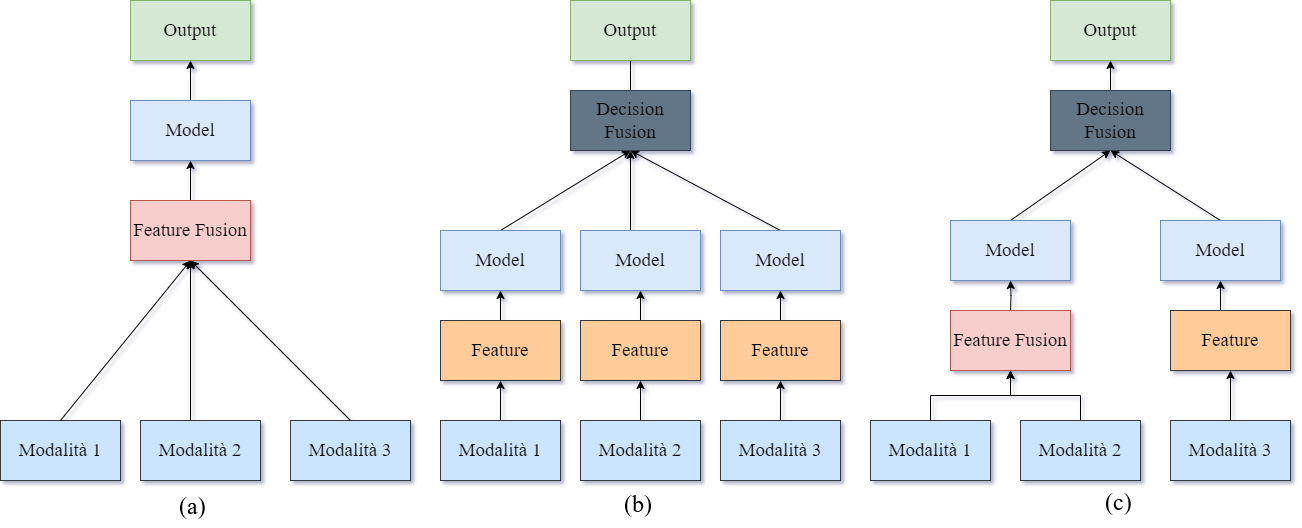
\includegraphics[width=\textwidth]{../../img/fusion_methods.png}
    \caption{Confronto tra i tre metodi di fusione. (a) Fusione basata su caratteristiche. (b) Fusione basata su decisioni. (c) Fusione Ibrida.}
    \label{fig:fusion_methods}
\end{figure}

In questo lavoro, \`e stato utilizzato un approccio di fusione basato su decisioni, in cui i modelli costruiti su codice sorgente e bytecode sono stati addestrati separatamente e le decisioni di entrambi i modelli sono state combinate per addestrare un meta-classificatore che fornisce il risultato finale. 

Questo approccio \`e stato testato con differenti modelli utilizzati come meta-classificatori, tra cui un modello di regressione logistica, un modello di support vector machine, un modello di random forest, un decision tree, un modello bayesiano ed un modello Gradient Boost. Tutti i modelli sono stati addestrati utilizzando la libreria Scikit-learn e l'API MultiOutputClassifier, che permette di addestrare un classificatore multilabel  e sono stati tunati gli iperparametri specifici di ogni modello utilizzando la funzione GridSearchCV con una cross-validation pari a 5.

I risultati ottenuti sono stati confrontati con i modelli costruiti su codice sorgente e bytecode per valutare l'efficacia dell'approccio di stacking.

\section{Gemini}
Al giorno d'oggi, chatbot basati su Large Language Models come Gemini e ChatGPT vengono sempre pi\`u spesso utilizzati come strumenti di supporto per le attivit\`a di tutti i giorni, come la ricerca di informazioni, la creazione di contenuti e la gestione delle attivit\`a quotidiane. Lo sviluppo software non si esime da questa tendenza, e sempre pi\`u spesso si fa ricorso a chatbot per la gestione di task di programmazione e sviluppo software sempre pi\`u complessi. Data l'importanza che questi strumenti stanno assumendo nelle nostre vite \`e importante valutarne le performance e la qualit\`a. Diventa quindi importante confrontare i modelli costruiti in questo lavoro di tesi con modelli gi\`a esistenti e ampiamente utilizzati come Gemini e ChatGPT.

Gemini \`e una famiglia di large language model multimodali sviluppato da Deep Mind Google, l'azienda fondata nel 2010 con sede a Londra che ha il compito di fare ricerca e sviluppo nel campo dell'intelligenza artificiale \cite{DeepMind}. 
Questa famiglia di modelli, \`e nata come successore di LaMDA e PaLM2, e comprende Gemini Ultra, Gemini Pro e Gemini Nano. Questi modelli sono stati poi resi famosi per dar vita al chatbot Gemini di Google, che si pone come principale competitor di GPT-4 di OpenAI \cite{Gemini}. 

La prima generazione di Gemini (``Gemini 1") ha tre modelli, con la stessa architettura software. Si tratta di transformer solo-decoder. Hanno una lunghezza del contesto di 32768 token. Sono poi state distillare due versioni di Gemini Nano: Nano-1 con 1,8 miliardi di parametri e Nano-2 avente 3,25 miliardi di parametri. Questi modelli sono distillati da modelli Gemini pi\`u grandi, progettati per l'uso da parte di dispositivi con potenza di calcolo limitata come gli smartphone. Poich\`e Gemini \`e multimodale, ogni finestra di contesto pu\`o contenere pi\`u forme di input. Le diverse modalit\`a possono essere interlacciate e non devono essere presentate in un ordine fisso, consentendo una conversazione multimodale. Ad esempio, l'utente potrebbe aprire la conversazione con una miscela di testo, immagini, video e audio, presentata in qualsiasi ordine e Gemini potrebbe rispondere con lo stesso ordine libero.

Il dataset di Gemini \`e multimodale e multilingue, composto da ``documenti web, libri e codice, e include dati di immagini, audio e video".

La seconda generazione di Gemini (``Gemini 1.5") ha due modelli pubblicati finora:
\begin{itemize}
    \item \emph{Gemini 1.5 Pro}: si tratta di un mixture-of-expertise sparso multimodale.
    \item \emph{Gemini 1.5 Flash}: un modello distillato da Gemini 1.5 Pro, con una lunghezza del contesto superiore a 2 milioni.
\end{itemize}


Per valutare quanto i modelli costruiti in questo lavoro siano performanti rispetto a chatbot disponibili online gratuitamente (o in versioni Pro a pagamento) come ChatGPT e Gemini \`e stata utilizzata la versione gratuita delle API di Gemini 1.5 Flash per testarlo in un task di classificazione multilabel delle vulnerabilit\`a degli smart contracts. Non \`e stato possibile effettuare gli stessi test utilizzando le API di ChatGPT in quanto esse non sono disponibili in forma di prova gratuita.

Il campione di dati raccolto per la valutazione del modello Gemini 1.5 Flash, \`e composto da 1169 elementi a  partire dal dataset di test. Questo \`e stato utilizzato come indicazione delle performance del modello rispetto ai modelli costruiti in questo lavoro. Non \`e stato possibile raccogliere un campione di dati pi\`u ampio (come ad esempio l'intero dataset di test) a causa delle limitazioni della versione gratuita delle API. 

Il prompt utilizzato per la valutazione di Gemini 1.5 Flash \`e stato scritto in lingua inglese e recita: 

\begin{quote}
Analyze the following smart contract for the presence of the following vulnerabilities:

access-control 

arithmetic

other

reentrancy

unchecked-calls

Reply ONLY with an array of 5 elements where each element is either 0 or 1. A 1 indicates the presence of the corresponding vulnerability, and a 0 indicates its absence.

For example, if the contract has arithmetic and reentrancy vulnerabilities, the output should be [0,1,0,1,0].
\end{quote}   
A questo prompt veniva concatenato la stringa del codice sorgente del contratto da analizzare, opportunamente gi\`a preprocessato con le stesse tecniche utilizzate per i modelli descritti in precedenza, quindi la rimozione dei commenti e delle funzioni getter monoistruzione. Mostriamo quindi un esempio di codice per l'utilizzo delle API di Gemini 1.5 Flash:
\begin{python}
import pathlib
import textwrap

import google.generativeai as genai

from IPython.display import display
from IPython.display import Markdown
from google.colab import userdata
GOOGLE_API_KEY=userdata.get('GOOGLE_API_KEY')

genai.configure(api_key=GOOGLE_API_KEY)
model = genai.GenerativeModel('gemini-1.5-flash')
response = model.generate_content(basePrompt + sourceCode)
\end{python}

Come si pu\`o notare nel codice sopra riportato, l'utilizzo del modello Gemini 1.5 Flash \`e estremamente semplice e intuitivo. Dopo aver configurato l'API key, si crea un oggetto di tipo GenerativeModel passando come parametro il nome del modello, in questo caso ``gemini-1.5-flash". Successivamente, si chiama il metodo generate\_content passando come parametro il prompt da utilizzare per la generazione del testo. Il risultato della chiamata al metodo generate\_content \`e un oggetto di tipo GenerativeModelResponse che contiene il testo generato dal modello. 
Il testo generato \`e stato controllato per assicurarsi che la generazione abbia prodotto solo un array di 5 elementi, ognuno dei quali \`e 0 o 1, come richiesto dal prompt. Questo \`e risultato vero per tutti i 1169 elementi del campione di dati. Successivamente, \`e stato convertito il testo generato in un array di 5 elementi, ognuno dei quali \`e 0 o 1, per poter calcolare le metriche di valutazione.
\end{document}
